\documentclass[a4paper]{article}\usepackage[]{graphicx}\usepackage[]{color}
%% maxwidth is the original width if it is less than linewidth
%% otherwise use linewidth (to make sure the graphics do not exceed the margin)
\makeatletter
\def\maxwidth{ %
  \ifdim\Gin@nat@width>\linewidth
    \linewidth
  \else
    \Gin@nat@width
  \fi
}
\makeatother

\definecolor{fgcolor}{rgb}{0.345, 0.345, 0.345}
\newcommand{\hlnum}[1]{\textcolor[rgb]{0.686,0.059,0.569}{#1}}%
\newcommand{\hlstr}[1]{\textcolor[rgb]{0.192,0.494,0.8}{#1}}%
\newcommand{\hlcom}[1]{\textcolor[rgb]{0.678,0.584,0.686}{\textit{#1}}}%
\newcommand{\hlopt}[1]{\textcolor[rgb]{0,0,0}{#1}}%
\newcommand{\hlstd}[1]{\textcolor[rgb]{0.345,0.345,0.345}{#1}}%
\newcommand{\hlkwa}[1]{\textcolor[rgb]{0.161,0.373,0.58}{\textbf{#1}}}%
\newcommand{\hlkwb}[1]{\textcolor[rgb]{0.69,0.353,0.396}{#1}}%
\newcommand{\hlkwc}[1]{\textcolor[rgb]{0.333,0.667,0.333}{#1}}%
\newcommand{\hlkwd}[1]{\textcolor[rgb]{0.737,0.353,0.396}{\textbf{#1}}}%

\usepackage{framed}
\makeatletter
\newenvironment{kframe}{%
 \def\at@end@of@kframe{}%
 \ifinner\ifhmode%
  \def\at@end@of@kframe{\end{minipage}}%
  \begin{minipage}{\columnwidth}%
 \fi\fi%
 \def\FrameCommand##1{\hskip\@totalleftmargin \hskip-\fboxsep
 \colorbox{shadecolor}{##1}\hskip-\fboxsep
     % There is no \\@totalrightmargin, so:
     \hskip-\linewidth \hskip-\@totalleftmargin \hskip\columnwidth}%
 \MakeFramed {\advance\hsize-\width
   \@totalleftmargin\z@ \linewidth\hsize
   \@setminipage}}%
 {\par\unskip\endMakeFramed%
 \at@end@of@kframe}
\makeatother

\definecolor{shadecolor}{rgb}{.97, .97, .97}
\definecolor{messagecolor}{rgb}{0, 0, 0}
\definecolor{warningcolor}{rgb}{1, 0, 1}
\definecolor{errorcolor}{rgb}{1, 0, 0}
\newenvironment{knitrout}{}{} % an empty environment to be redefined in TeX

\usepackage{alltt}

\usepackage[utf8]{inputenc}
\usepackage{fullpage}
\usepackage{amsmath}
\DeclareMathOperator*{\argmin}{arg\,min}
\DeclareMathOperator*{\argmax}{arg\,max}
\title{STK9030 – Semester project}
\author{Candidate number: 1}
\date{\today}
\IfFileExists{upquote.sty}{\usepackage{upquote}}{}
\begin{document}

\maketitle

This is my report for the mandatory project in STK9030. Some code and output is included in the text, but most of the code, especially for figures and calculations, is collected in the appendix.

\section{\emph{Vino Verde} wine quality}

We start by loading the needed libraries and data, and standardizing all the covariates.



\subsection{OLS}
We then fit an ordinary least squares model on the training set, and predict the quality of the test set.

\begin{knitrout}
\definecolor{shadecolor}{rgb}{0.969, 0.969, 0.969}\color{fgcolor}\begin{kframe}
\begin{alltt}
\hlstd{fit} \hlkwb{<-} \hlkwd{lm}\hlstd{(quality}\hlopt{~}\hlstd{.,} \hlkwc{data}\hlstd{=train)}
\hlstd{pred} \hlkwb{<-} \hlkwd{predict}\hlstd{(fit, test)}
\end{alltt}
\end{kframe}
\end{knitrout}

The coefficients are as follows
\begin{knitrout}
\definecolor{shadecolor}{rgb}{0.969, 0.969, 0.969}\color{fgcolor}\begin{kframe}
\begin{alltt}
\hlstd{fit}\hlopt{$}\hlstd{coefficients}
\end{alltt}
\begin{verbatim}
##          (Intercept)        fixed.acidity     volatile.acidity 
##           5.97752609           0.07909568          -0.24270090 
##          citric.acid       residual.sugar            chlorides 
##          -0.06274916           0.39028402           0.10741013 
##  free.sulfur.dioxide total.sulfur.dioxide              density 
##           0.15437016          -0.08263811          -0.26150564 
##                   pH            sulphates              alcohol 
##           0.06431949           0.04545207           0.43090830
\end{verbatim}
\end{kframe}
\end{knitrout}
The test error (root mean squared error) is 0.7651927, which seems pretty good for a response variable in the range 0 to 10.

Inspecting the summary of the model we see that the variables most correlated to the quality (in the OLS model) are \texttt{alcohol}, \texttt{volatile acidity} and \texttt{residual sugar}.

\subsection{Ridge}

We use the \texttt{glmnet} package to perform Ridge regression, by setting the \texttt{alpha} parameter to zero. The package has built in cross-validation functionality which we use to find the best $\lambda$ parameter.


Figure \ref{fig:ridge_lambda} shows a plot of the mean squared error against the base 10 logarithm of the $\lambda$ values tested in the cross-validation.
\begin{knitrout}
\definecolor{shadecolor}{rgb}{0.969, 0.969, 0.969}\color{fgcolor}\begin{figure}
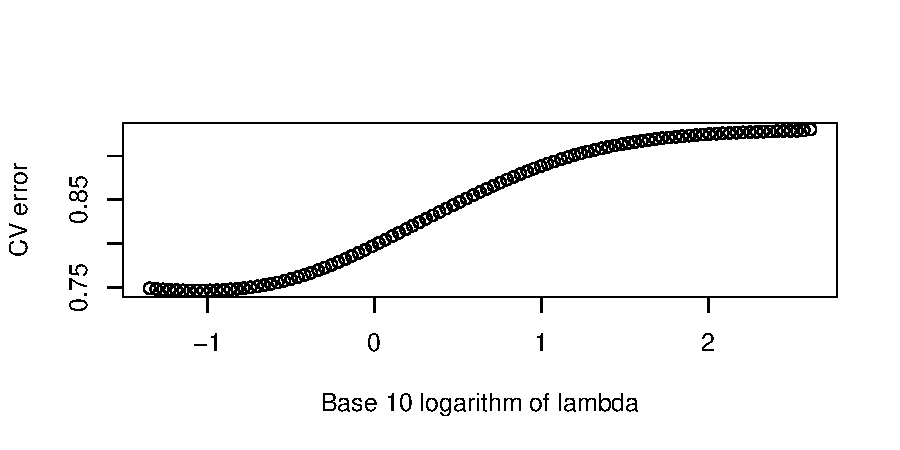
\includegraphics[width=\maxwidth]{figure/ridge_lambda-1} \caption[The mean squared error against the base 10 logarithm of the ]{The mean squared error against the base 10 logarithm of the $\lambda$ parameter for Ridge regression.}\label{fig:ridge_lambda}
\end{figure}


\end{knitrout}
The $\lambda$ parameter giving the smallest cross-validation error is returned by \texttt{glmnet} in the \texttt{lambda.min} variable, and is 0.1141166. The coefficients of the regression model are
\begin{knitrout}
\definecolor{shadecolor}{rgb}{0.969, 0.969, 0.969}\color{fgcolor}\begin{kframe}
\begin{alltt}
\hlstd{ridgefit}\hlopt{$}\hlstd{beta}
\end{alltt}
\begin{verbatim}
## 11 x 1 sparse Matrix of class "dgCMatrix"
##                               s0
## fixed.acidity         0.02664548
## volatile.acidity     -0.20442628
## citric.acid          -0.04325901
## residual.sugar        0.20670174
## chlorides             0.04030215
## free.sulfur.dioxide   0.12795671
## total.sulfur.dioxide -0.07249421
## density              -0.10450824
## pH                    0.03033831
## sulphates             0.03013614
## alcohol               0.38839485
\end{verbatim}
\end{kframe}
\end{knitrout}

The root mean square error on the test data becomes
\begin{knitrout}
\definecolor{shadecolor}{rgb}{0.969, 0.969, 0.969}\color{fgcolor}\begin{kframe}
\begin{alltt}
\hlstd{pred} \hlkwb{<-} \hlkwd{predict}\hlstd{(ridgefit,} \hlkwd{as.matrix}\hlstd{(test[,}\hlnum{1}\hlopt{:}\hlnum{11}\hlstd{]))}
\hlkwd{sqrt}\hlstd{(}\hlkwd{mean}\hlstd{((pred} \hlopt{-} \hlstd{test[,}\hlstr{'quality'}\hlstd{])}\hlopt{^}\hlnum{2}\hlstd{))}
\end{alltt}
\begin{verbatim}
## [1] 0.7488399
\end{verbatim}
\end{kframe}
\end{knitrout}

\subsection{Lasso}
We use the \texttt{glmnet} in the same way as we did for Ridge regression. We now have to set the elastic net parameter $\alpha$ to 1, so obtain a Lasso regression. We also here use \texttt{glmnet}s built-in cross-validation features.


Figure \ref{fig:lasso_lambda} shows a plot of the mean squared error against the base 10 logarithm of the $\lambda$ values tested in the cross-validation.
\begin{knitrout}
\definecolor{shadecolor}{rgb}{0.969, 0.969, 0.969}\color{fgcolor}\begin{figure}
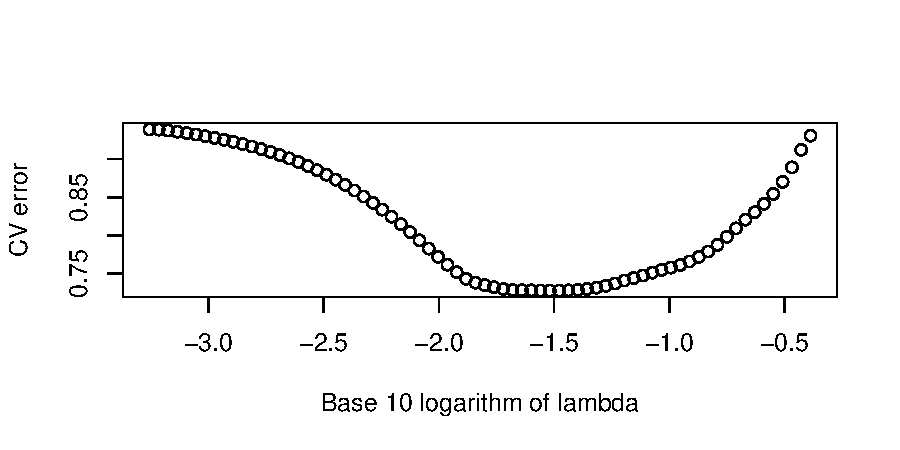
\includegraphics[width=\maxwidth]{figure/lasso_lambda-1} \caption[The mean squared error against the base 10 logarithm of the ]{The mean squared error against the base 10 logarithm of the $\lambda$ parameter for the Lasso regression.}\label{fig:lasso_lambda}
\end{figure}


\end{knitrout}
The $\lambda$ giving the smallest cross-validation error is 0.0303104 and the coefficients are
\begin{knitrout}
\definecolor{shadecolor}{rgb}{0.969, 0.969, 0.969}\color{fgcolor}\begin{kframe}
\begin{alltt}
\hlstd{lassofit}\hlopt{$}\hlstd{beta}
\end{alltt}
\begin{verbatim}
## 11 x 1 sparse Matrix of class "dgCMatrix"
##                                s0
## fixed.acidity         .          
## volatile.acidity     -0.212441153
## citric.acid          -0.004175180
## residual.sugar        0.109787082
## chlorides             .          
## free.sulfur.dioxide   0.081221067
## total.sulfur.dioxide -0.006324578
## density               .          
## pH                    .          
## sulphates             .          
## alcohol               0.445281056
\end{verbatim}
\end{kframe}
\end{knitrout}
We note that five of the coefficients have been constrained to zero, a property of the $L_1$ penalty in the Lasso regression.

The mean square error becomes
\begin{knitrout}
\definecolor{shadecolor}{rgb}{0.969, 0.969, 0.969}\color{fgcolor}\begin{kframe}
\begin{alltt}
\hlstd{pred} \hlkwb{<-} \hlkwd{predict}\hlstd{(lassofit,} \hlkwd{as.matrix}\hlstd{(test[,}\hlnum{1}\hlopt{:}\hlnum{11}\hlstd{]))}
\hlkwd{sqrt}\hlstd{(}\hlkwd{mean}\hlstd{((pred} \hlopt{-} \hlstd{test[,}\hlstr{'quality'}\hlstd{])}\hlopt{^}\hlnum{2}\hlstd{))}
\end{alltt}
\begin{verbatim}
## [1] 0.7445097
\end{verbatim}
\end{kframe}
\end{knitrout}
Slightly lower than the Ridge regression error.

\subsection{Comparison}

We see that the Lasso regression has a slightly lower mean squared error on the test set compared to the OLS and the Ridge regression. In addition the Lasso method set five of the 11 coefficients to zero, meaning it explains the response accurately, using fewest covariates. This can be seen as an advantage.

Based on this I would recommend the wine seller to use the Lasso regression. By selecting the best of three methods based on the test set performance we have basically fitted our model slightly to the test set, meaning we can not expect the error on our test set to be a good unbiased estimate of the true test error.

\section{Fossils}

We load the fossils dataset, which contains the
\texttt{strontium.ratio} and
\texttt{age}
of 106 fossil samples. 


\subsection{Spline basis}

We construct two different cubic B-spline basises, differing in the way we place the internal knots. The boundary knots are placed at the extremes of the \texttt{age} variable, with 40 internal knots in between. First we construct a knot vector with equidistant knots, with distance 0.761 between the knots. We use the \texttt{bs} function of the \texttt{spline} package in R, and the results are shown in Figure~\ref{fig:equal_cubic}.

\begin{knitrout}
\definecolor{shadecolor}{rgb}{0.969, 0.969, 0.969}\color{fgcolor}\begin{figure}
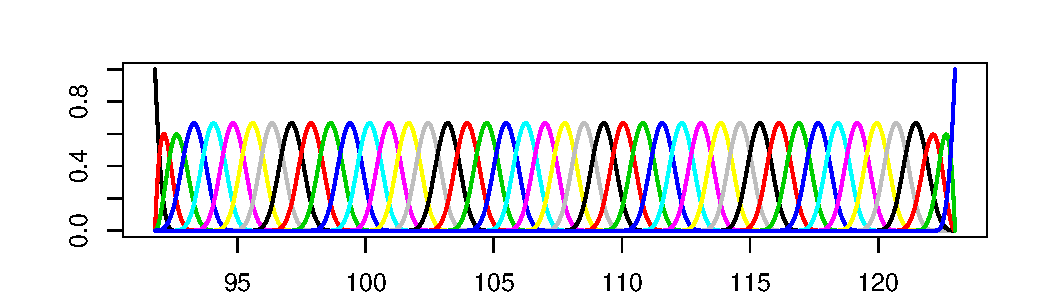
\includegraphics[width=\maxwidth]{figure/equal_cubic-1} \caption[Cubic splines with equal knot spacing and 40 internal knots]{Cubic splines with equal knot spacing and 40 internal knots.}\label{fig:equal_cubic}
\end{figure}


\end{knitrout}

We construct another B-spline basis with a knot vector with the same number of knots, but where they are placed at equidistant quantiles of the distribution of \texttt{age}. The resulting basis is shown in Figure~\ref{fig:quantile_cubic}. We note that in areas of the \texttt{age} range where we have many points (see Figure~\ref{fig:smooth_fossil}), we have a more refined basis.

\begin{knitrout}
\definecolor{shadecolor}{rgb}{0.969, 0.969, 0.969}\color{fgcolor}\begin{figure}
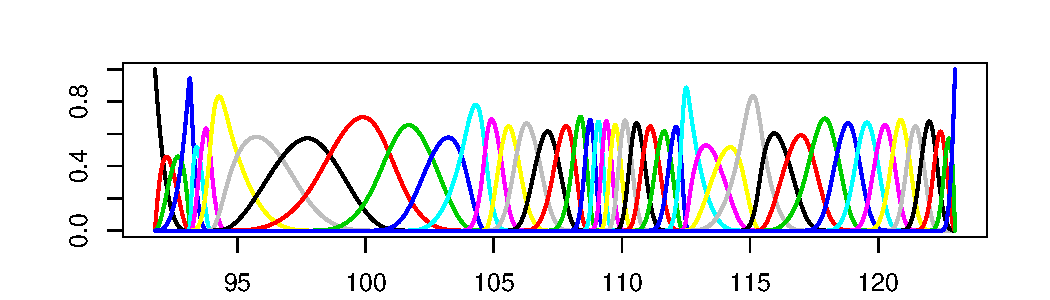
\includegraphics[width=\maxwidth]{figure/quantile_cubic-1} \caption[Cubic splines with quantile knot spacing and 40 internal knots]{Cubic splines with quantile knot spacing and 40 internal knots.}\label{fig:quantile_cubic}
\end{figure}


\end{knitrout}

\subsection{Smoothing splines}

Using the quantile B-spline basis we estimate a smoothing spline regression curve for our data. The smoothing spline includes a parameter $\lambda$ which restricts the second derivative of the spline. In theory we seek a function $f(x)$ minimizing
\begin{equation}
\sum_{i=1}^N (y_i - f(x_i))^2 + \lambda \int (f''(t))^2 dt.
\end{equation}
This has a unique solution which is a natural cubic spline with knots at all values of $x$, but in practice it is easier to use a B-spline basis, resulting in what is sometimes called \emph{penalized splines}. We use the \texttt{smooth.spline} function in R to estimate the smoothing spline. Through the \texttt{nknots} parameter we can control the number of knots, which are placed at the quantiles of $x$, so we set this to 42 for 40 internal knots and two boundary knots. We can verify that it uses the same knots as in our constructed basis by looking at the returned \texttt{smoothing\_ocv\$fit\$knot} vector. This vector in addition includes repeated boundary knots which restricts the second and higher derivatives at the boundary to zero.
\begin{knitrout}
\definecolor{shadecolor}{rgb}{0.969, 0.969, 0.969}\color{fgcolor}\begin{kframe}
\begin{alltt}
\hlstd{smoothing_ocv} \hlkwb{<-} \hlkwd{smooth.spline}\hlstd{(fossil}\hlopt{$}\hlstd{age, fossil}\hlopt{$}\hlstd{strontium.ratio,} \hlkwc{nknots}\hlstd{=}\hlnum{42}\hlstd{,} \hlkwc{cv}\hlstd{=}\hlnum{TRUE}\hlstd{)}
\hlstd{smoothing_gcv} \hlkwb{<-} \hlkwd{smooth.spline}\hlstd{(fossil}\hlopt{$}\hlstd{age, fossil}\hlopt{$}\hlstd{strontium.ratio,} \hlkwc{nknots}\hlstd{=}\hlnum{42}\hlstd{,} \hlkwc{cv}\hlstd{=}\hlnum{FALSE}\hlstd{)}
\end{alltt}
\end{kframe}
\end{knitrout}
The \texttt{cv} parameter of \texttt{smooth.spline} controls whether we want to use ordinary (\texttt{TRUE}) or generalized (\texttt{FALSE}) cross-validation. The smoothing parameters giving the smallest cross-validation score can be found in the \texttt{spar} variable:
\begin{knitrout}
\definecolor{shadecolor}{rgb}{0.969, 0.969, 0.969}\color{fgcolor}\begin{kframe}
\begin{alltt}
\hlstd{smoothing_ocv}\hlopt{$}\hlstd{spar}
\end{alltt}
\begin{verbatim}
## [1] 0.5616376
\end{verbatim}
\begin{alltt}
\hlstd{smoothing_gcv}\hlopt{$}\hlstd{spar}
\end{alltt}
\begin{verbatim}
## [1] 0.5771304
\end{verbatim}
\end{kframe}
\end{knitrout}
Note that this is not \emph{equal to}, but \emph{a function of} $\lambda$. We see from the values, and from the plot of the smoothing splines over the data in Figure~\ref{fig:smooth_fossil} that these smoothing parameters are equal for all intents and purposes.
\begin{knitrout}
\definecolor{shadecolor}{rgb}{0.969, 0.969, 0.969}\color{fgcolor}\begin{figure}
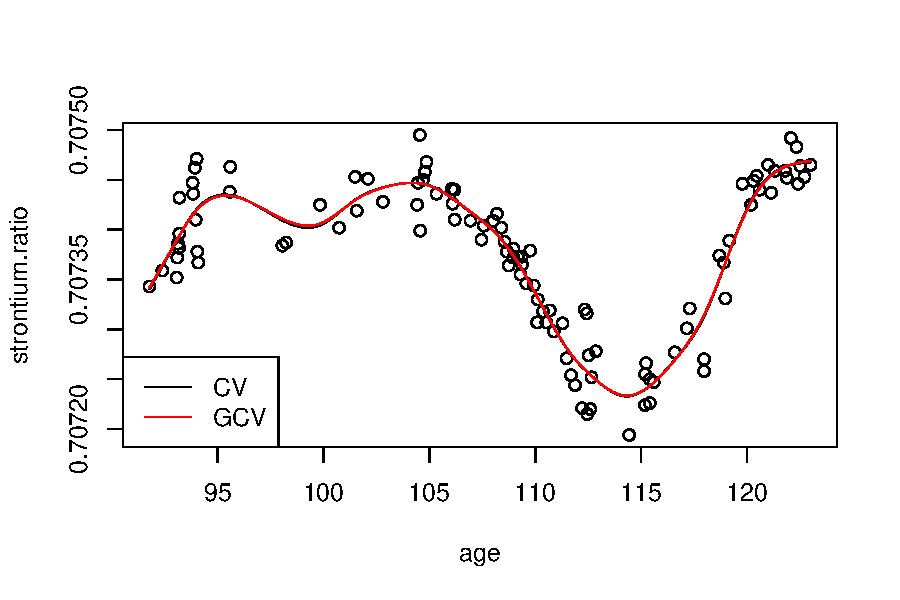
\includegraphics[width=\maxwidth]{figure/smooth_fossil-1} \caption[The fossil data with smoothing splines]{The fossil data with smoothing splines.}\label{fig:smooth_fossil}
\end{figure}


\end{knitrout}
The predicted strontium ratio for an 113.5 million years old fossil then becomes
\begin{knitrout}
\definecolor{shadecolor}{rgb}{0.969, 0.969, 0.969}\color{fgcolor}\begin{kframe}
\begin{alltt}
\hlkwd{predict}\hlstd{(smoothing_gcv,} \hlkwd{c}\hlstd{(}\hlnum{113.5}\hlstd{))}\hlopt{$}\hlstd{y}
\end{alltt}
\begin{verbatim}
## [1] 0.7072393
\end{verbatim}
\end{kframe}
\end{knitrout}

\section{Face recognition}



We begin by loading the face images, and the \texttt{shoulder} vector. The provided \texttt{display.matrix.r} is used to display the 10000 pixel vectors in a square plot.

\subsection{Mean images}

First we calculate the mean images. Figure~\ref{fig:mean_gender} shows the mean male and female images. The difference in hair length is clearly visible. We know that some images are only the face, while others include the shoulders. This also shows in the mean images.
\begin{knitrout}
\definecolor{shadecolor}{rgb}{0.969, 0.969, 0.969}\color{fgcolor}\begin{figure}
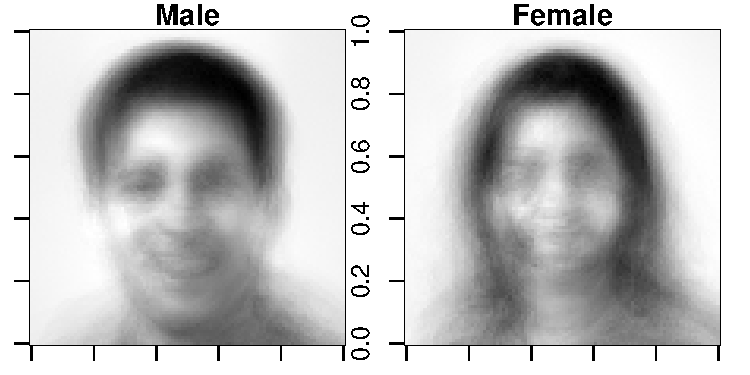
\includegraphics[width=\maxwidth]{figure/mean_gender-1} \caption[Mean subset of images from each gender]{Mean subset of images from each gender.}\label{fig:mean_gender}
\end{figure}


\end{knitrout}

\subsection{Principal components}

We calculate the principal components using the R function \texttt{prcomp}, which also centers and scales the features for us to have zero mean and unit variance (where one feature is now one pixel position). 
\begin{knitrout}
\definecolor{shadecolor}{rgb}{0.969, 0.969, 0.969}\color{fgcolor}\begin{kframe}
\begin{alltt}
\hlstd{eigenfaces} \hlkwb{<-} \hlkwd{prcomp}\hlstd{(}\hlkwd{t}\hlstd{(faces),} \hlkwc{center}\hlstd{=}\hlnum{TRUE}\hlstd{,} \hlkwc{scale}\hlstd{=}\hlnum{TRUE}\hlstd{)}
\end{alltt}
\end{kframe}
\end{knitrout}

The first four principal component directions (eigenvectors) are shown in Figure~\ref{fig:pca_1_4}. We note the eigenvectors indicate directions of variation, and thus ``dark'' and ``bright'' can be flipped in these pictures without affecting the results. The first vector seems to be a direction separating foreground and background, which is understandable, as all the images has face and background in approximately the same areas. The second component seems to be a long hair feature, while the third component captures short hair variation.
\begin{knitrout}
\definecolor{shadecolor}{rgb}{0.969, 0.969, 0.969}\color{fgcolor}\begin{figure}
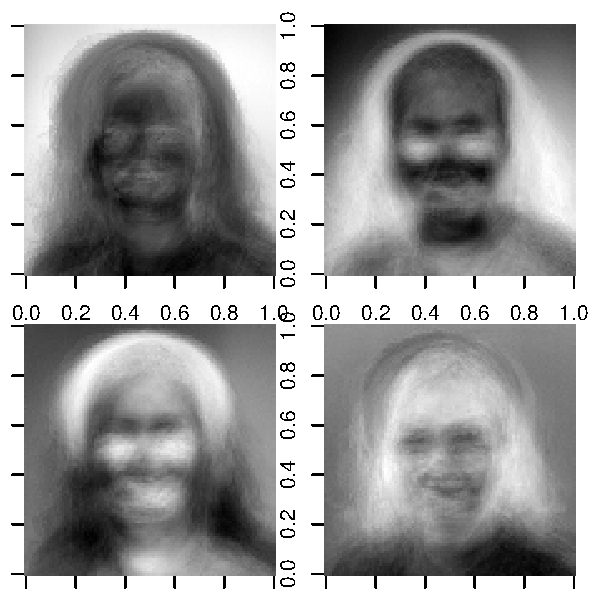
\includegraphics[width=\maxwidth]{figure/pca_1_4-1} \caption[First four principal component directions]{First four principal component directions.}\label{fig:pca_1_4}
\end{figure}


\end{knitrout}

Here is a list of the cumulative proportion of variance explained for the components 37 to 43, and we see that we need 39 components to explain 80\% of the variation in the images.
\begin{knitrout}
\definecolor{shadecolor}{rgb}{0.969, 0.969, 0.969}\color{fgcolor}\begin{kframe}
\begin{alltt}
\hlkwd{summary}\hlstd{(eigenfaces)}\hlopt{$}\hlstd{importance[}\hlnum{3}\hlstd{,} \hlnum{37}\hlopt{:}\hlnum{43}\hlstd{]}
\end{alltt}
\begin{verbatim}
##    PC37    PC38    PC39    PC40    PC41    PC42    PC43 
## 0.79324 0.79682 0.80033 0.80379 0.80715 0.81041 0.81365
\end{verbatim}
\end{kframe}
\end{knitrout}

\subsection{First principal components vs.\ gender and shoulders}

\begin{knitrout}
\definecolor{shadecolor}{rgb}{0.969, 0.969, 0.969}\color{fgcolor}\begin{figure}

{\centering 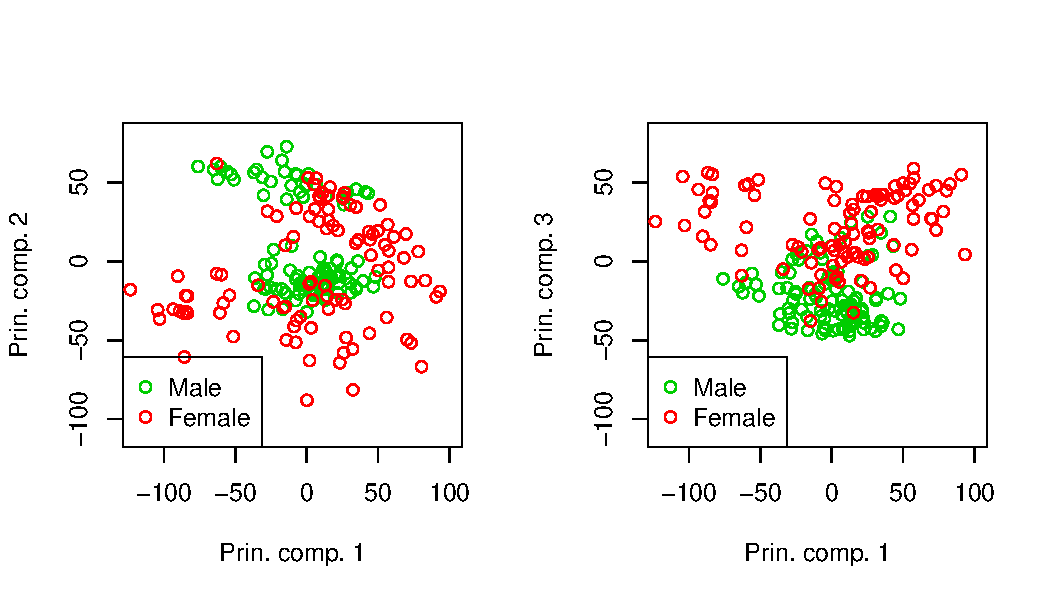
\includegraphics[width=\maxwidth]{figure/gender_components-1} 

}

\caption[First three principal components of the females and males]{First three principal components of the females and males.}\label{fig:gender_components}
\end{figure}


\end{knitrout}

We plot the first and second, and first and third principal components of our samples against eachother, and color the points according to the gender of the person. This is shown in Figure~\ref{fig:gender_components}. We observe that the female images show higher variation in the first principal components, while the male images are more concentrated, possibly caused by hair length and also the shoulder variation. We further note that out of the three components, the third principal component seems to be the most useful for classifying gender, and the first component the least useful. This corresponds well to Figure~\ref{fig:pca_1_4}, where we observed that the second and third components have a lot to do with hair variation.

\begin{knitrout}
\definecolor{shadecolor}{rgb}{0.969, 0.969, 0.969}\color{fgcolor}\begin{figure}
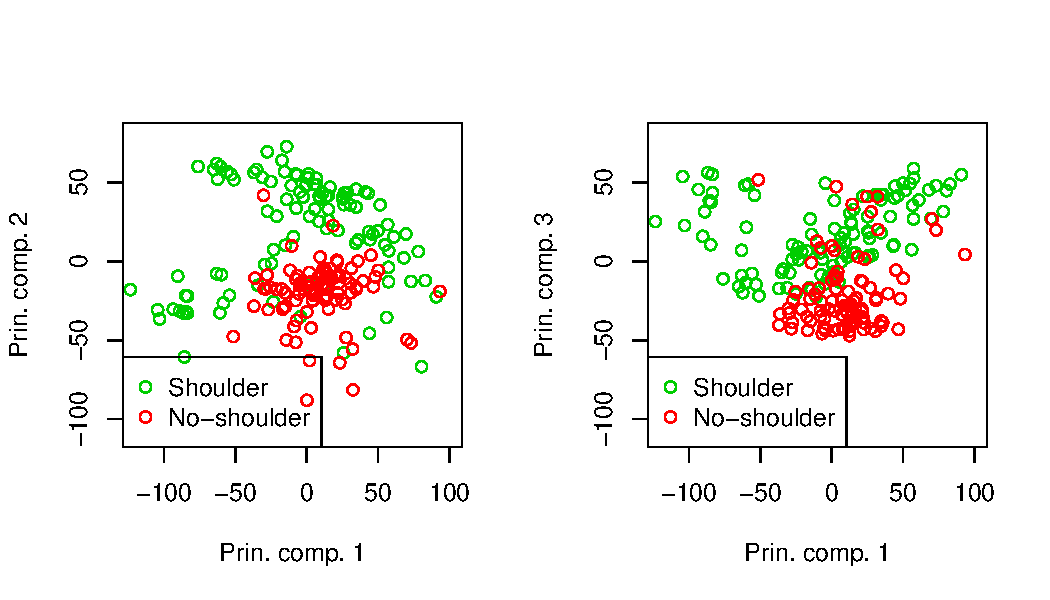
\includegraphics[width=\maxwidth]{figure/shoulder_components-1} \caption[First three principal components of the shoulder and no-shoulder pictures]{First three principal components of the shoulder and no-shoulder pictures.}\label{fig:shoulder_components}
\end{figure}


\end{knitrout}

Similarly we plot the first three principal components in Figure~\ref{fig:shoulder_components}, coloring the points according to whether the image contains shoulders or not. We can observe similar trends, that the principal component number three is the most useful in separating shoulder from no-shoulder images. This similarity is probably related to the fact that there are 73 female images with shoulders, while only 34 male images with shoulders, so there is a correlation between the two variables.

\subsection{Principal component regression for gender classification}





Motivated by the previous visualizations we try to classify the gender by regression on $m$ of the 200 principal components. We encode the gender indicator $y_i$ as $-1$ for male and $1$ for female. A prediction $\hat{f}(x_i) > 0$ is classified as female. We use leave-one-out cross-validation to select a number $m$ of principal components that generalizes well without overfitting. Note that the principal components are only calculated once based on the whole training set, for speed. Although this could affect the results slightly, leaving one sample out should not really affect the first principal components much. We use a 1-0-loss, and choose the smallest $m$ if there are multiple minima. The result is $m = 22$ components.

Using this parameter we fit a model to all the training data. The misclassification rate on the training data becomes
\begin{knitrout}
\definecolor{shadecolor}{rgb}{0.969, 0.969, 0.969}\color{fgcolor}\begin{kframe}
\begin{alltt}
\hlkwd{sum}\hlstd{(pred} \hlopt{!=} \hlstd{gender)} \hlopt{/} \hlkwd{length}\hlstd{(pred)}
\end{alltt}
\begin{verbatim}
## [1] 0.075
\end{verbatim}
\end{kframe}
\end{knitrout}

\subsection{Partial least squares for gender classification}






Principal component regression seemed to work well. One problem though is that the first principal components are great for explaining the variation in the \emph{data}, but not necessarily variation in the response $y$. Partial least squares tries to improve on this by including the response $y$ in the procedure. We here use the \texttt{plsr} function from the \texttt{pls} package, which supports leave-one-out cross-validation. The object returned from \texttt{plsr} contains the cross-validation prediction of the left-out samples in the array \texttt{fit\$validation\$pred}. We use these predictions to calculate the 1-0-cross-validation error for each number of included components $m$. The number of components giving the lowest cross-validation error is $m = 9$, less than half of the number of components in principal components regression.

The \texttt{plsr} routine is optimized for speed and will only estimate the components of the model once. Recalculating the model ($\sim 10$ sec) for each $m < 200$ for each left-out sample (200) would take $200 * 200 * 10$ sec $\approx 111$ hours. The misclassification rate on the training data becomes
\begin{knitrout}
\definecolor{shadecolor}{rgb}{0.969, 0.969, 0.969}\color{fgcolor}\begin{kframe}
\begin{alltt}
\hlkwd{sum}\hlstd{(pred} \hlopt{!=} \hlstd{gender)} \hlopt{/} \hlkwd{length}\hlstd{(pred)}
\end{alltt}
\begin{verbatim}
## [1] 0
\end{verbatim}
\end{kframe}
\end{knitrout}
Much better than prinicpal component regression, with much fewer components! So it seems like the partial least squares routine managed to extract components more related to the response: gender. I imagine it dropped components containing information like ``face vs.\ background'' or ``eyes'' or ``shoulders'' as these are prominent things in the images, but also something that appears in both male and female images thus yielding little information regarding the gender.

\subsection{QDA + PCA for gender classification}



Since QDA does not work in the high-dimensional setting of 10000 pixels and only 200 images, we use instead the first 5 principal components of the 200 images as our data. We use the \texttt{qda} method included in the \texttt{MASS} package to create our QDA model. Figure~\ref{fig:qda_contours} shows the same plots as in Figure~\ref{fig:gender_components}, but now includes the QDA decision boundary. As our classes are coded as -1 and 1, we plot the boundary at $\hat{f}(x) = 0$. In 2D, the plots only have two axes, and the components included in the classification but not included in the plots are set to their mean value. Using color grading we could possibly have visualized one more dimension.

\begin{knitrout}
\definecolor{shadecolor}{rgb}{0.969, 0.969, 0.969}\color{fgcolor}\begin{figure}
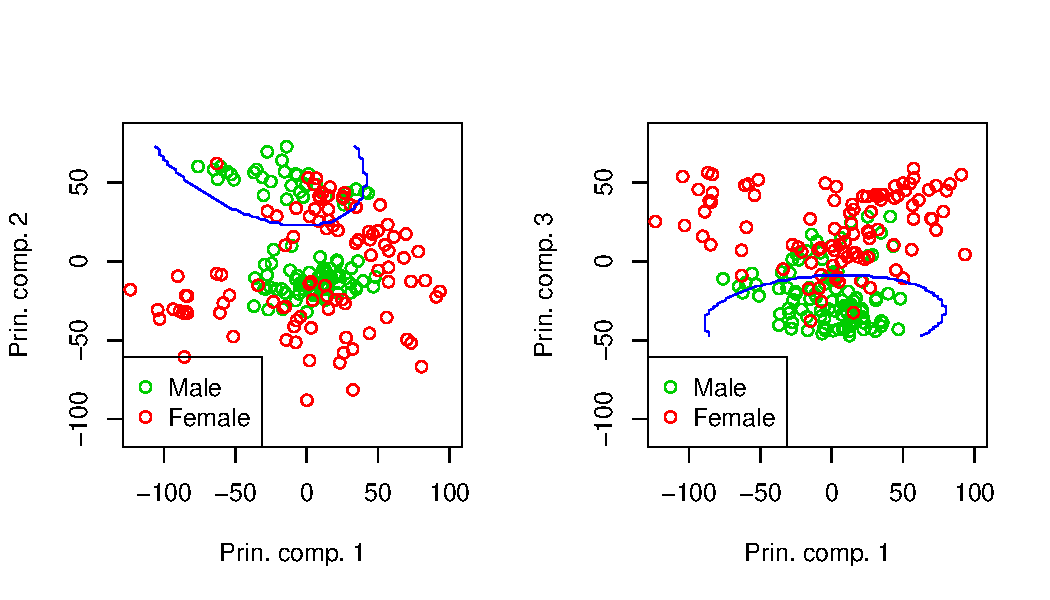
\includegraphics[width=\maxwidth]{figure/qda_contours-1} \caption[QDA contour at prediction 0 for first vs]{QDA contour at prediction 0 for first vs. second and first vs. third principal component. The not visible principal components have been set to their mean value.}\label{fig:qda_contours}
\end{figure}


\end{knitrout}

The misclassification rate on the training data for the QDA classifier becomes
\begin{knitrout}
\definecolor{shadecolor}{rgb}{0.969, 0.969, 0.969}\color{fgcolor}\begin{kframe}
\begin{alltt}
\hlstd{pred} \hlkwb{<-} \hlkwd{predict}\hlstd{(qfit, pdat)}\hlopt{$}\hlstd{class}
\hlkwd{sum}\hlstd{(pred} \hlopt{!=} \hlstd{gender)} \hlopt{/} \hlkwd{length}\hlstd{(pred)}
\end{alltt}
\begin{verbatim}
## [1] 0.085
\end{verbatim}
\end{kframe}
\end{knitrout}

\subsection{Multi-label QDA}

We augment the response variable by creating four different categories, males and females both with and without shoulders. Again we use the \texttt{qda} function of the \texttt{MASS} package as it can handle multiple categories.




After classifying the training data into these four categories we combine the results back into two categories, male and female. The misclassification rate on the training data is then
\begin{knitrout}
\definecolor{shadecolor}{rgb}{0.969, 0.969, 0.969}\color{fgcolor}\begin{kframe}
\begin{alltt}
\hlkwd{sum}\hlstd{(pg} \hlopt{!=} \hlstd{gender)} \hlopt{/} \hlkwd{length}\hlstd{(gender)}
\end{alltt}
\begin{verbatim}
## [1] 0.08
\end{verbatim}
\end{kframe}
\end{knitrout}
One more sample is classified correctly.

\subsection{Penalized LDA for gender classification}





Finally we return to the whole ($10000 \times 200$) dataset and use LDA as a combined dimension reduction and classification tool, by penalizing the covariance matrix. When doing LDA we usually assume that the samples come from some multivariate Gaussian distribution modeling the likelihood of class $\omega$ as
\begin{equation}
p(x \mid \omega) = \frac{1}{\sqrt{(2\pi)^p |\Sigma|}} \exp \left( -\frac{1}{2} (x - \mu_\omega)^T \Sigma^{-1} (x - \mu_\omega) \right).
\end{equation}
When we have a lot of data ($n > p$) we can estimate $\Sigma$ to be the sample covariance matrix. In our case the sample covariance matrix will be singular. One possibility is to set $\Sigma = I$, the identity matrix. This means that classification will be a simple comparison with the class means of male and female. Another possibility is to do something in-between, where we use a regularized covariance matrix
\begin{equation}
\Sigma_\gamma = \gamma \hat{\Sigma} + (1-\gamma) I.
\end{equation}
Using leave-one-out cross-validation, we estimate the regularization parameter $\gamma$. For 6 values between 0 and 0.6, we find 0.6 to give the minimal cross-validation misclassification rate at 0.09. For higher values of $\gamma$ I had trouble inverting the regularized covariance matrix.

The misclassification rate on the whole training set then becomes
\begin{knitrout}
\definecolor{shadecolor}{rgb}{0.969, 0.969, 0.969}\color{fgcolor}\begin{kframe}
\begin{alltt}
\hlstd{pred} \hlkwb{<-} \hlkwd{myLDA}\hlstd{(faces, faces, mm, fm, glist[}\hlkwd{which.max}\hlstd{(errs)])}
\hlkwd{sum}\hlstd{(pred} \hlopt{!=} \hlstd{gender)} \hlopt{/} \hlkwd{length}\hlstd{(pred)}
\end{alltt}
\begin{verbatim}
## [1] 0
\end{verbatim}
\end{kframe}
\end{knitrout}

In conclusion it seems that all these methods work pretty well on classifying the gender of the images in this setting where the setup, pose and position of the face is fairly standardized. More testing on a separate testing set would be needed to do a fair comparison between them.

\appendix
\section{\emph{Vino Verde} wine quality}

\begin{knitrout}
\definecolor{shadecolor}{rgb}{0.969, 0.969, 0.969}\color{fgcolor}\begin{kframe}
\begin{alltt}
\hlkwd{load}\hlstd{(}\hlstr{'wine.rdata'}\hlstd{)}
\hlstd{wine[,} \hlnum{1}\hlopt{:}\hlnum{11}\hlstd{]} \hlkwb{<-} \hlkwd{scale}\hlstd{(wine[,} \hlnum{1}\hlopt{:}\hlnum{11}\hlstd{])}
\hlstd{train} \hlkwb{<-} \hlstd{wine[wine[,} \hlstr{'test'}\hlstd{]} \hlopt{==} \hlnum{FALSE}\hlstd{,} \hlopt{-}\hlnum{13}\hlstd{]}
\hlstd{test} \hlkwb{<-} \hlstd{wine[wine[,} \hlstr{'test'}\hlstd{]} \hlopt{==} \hlnum{TRUE}\hlstd{,} \hlopt{-}\hlnum{13}\hlstd{]}
\end{alltt}
\end{kframe}
\end{knitrout}

\subsection{Ridge regression}

\begin{knitrout}
\definecolor{shadecolor}{rgb}{0.969, 0.969, 0.969}\color{fgcolor}\begin{kframe}
\begin{alltt}
\hlkwd{library}\hlstd{(glmnet)}
\hlstd{cvridge} \hlkwb{<-} \hlkwd{cv.glmnet}\hlstd{(}\hlkwd{as.matrix}\hlstd{(train[,}\hlnum{1}\hlopt{:}\hlnum{11}\hlstd{]),} \hlkwd{as.matrix}\hlstd{(train[,}\hlnum{12}\hlstd{]),}
                     \hlkwc{alpha}\hlstd{=}\hlnum{0}\hlstd{,} \hlkwc{family}\hlstd{=}\hlstr{'gaussian'}\hlstd{,}
                     \hlkwc{standardize}\hlstd{=}\hlnum{FALSE}\hlstd{,} \hlkwc{type.measure}\hlstd{=}\hlstr{'mse'}\hlstd{,} \hlkwc{nfolds}\hlstd{=}\hlnum{10}\hlstd{)}

\hlstd{ridgefit} \hlkwb{<-} \hlkwd{glmnet}\hlstd{(}\hlkwd{as.matrix}\hlstd{(train[,}\hlnum{1}\hlopt{:}\hlnum{11}\hlstd{]),} \hlkwd{as.matrix}\hlstd{(train[,}\hlnum{12}\hlstd{]),}
                     \hlkwc{alpha}\hlstd{=}\hlnum{0}\hlstd{,} \hlkwc{family}\hlstd{=}\hlstr{'gaussian'}\hlstd{,}
                     \hlkwc{standardize}\hlstd{=}\hlnum{FALSE}\hlstd{,} \hlkwc{lambda}\hlstd{=cvridge}\hlopt{$}\hlstd{lambda.min)}
\end{alltt}
\end{kframe}
\end{knitrout}

\begin{knitrout}
\definecolor{shadecolor}{rgb}{0.969, 0.969, 0.969}\color{fgcolor}\begin{kframe}
\begin{alltt}
\hlkwd{plot}\hlstd{(}\hlkwd{log}\hlstd{(cvridge}\hlopt{$}\hlstd{lambda,} \hlnum{10}\hlstd{), cvridge}\hlopt{$}\hlstd{cvm,}
     \hlkwc{xlab}\hlstd{=}\hlstr{"Base 10 logarithm of lambda"}\hlstd{,} \hlkwc{ylab}\hlstd{=}\hlstr{"CV error"}\hlstd{)}
\end{alltt}
\end{kframe}
\end{knitrout}

\subsection{Lasso regression}

\begin{knitrout}
\definecolor{shadecolor}{rgb}{0.969, 0.969, 0.969}\color{fgcolor}\begin{kframe}
\begin{alltt}
\hlkwd{library}\hlstd{(glmnet)}
\hlstd{cvlasso} \hlkwb{<-} \hlkwd{cv.glmnet}\hlstd{(}\hlkwd{as.matrix}\hlstd{(train[,}\hlnum{1}\hlopt{:}\hlnum{11}\hlstd{]),} \hlkwd{as.matrix}\hlstd{(train[,}\hlnum{12}\hlstd{]),}
                     \hlkwc{alpha}\hlstd{=}\hlnum{1}\hlstd{,} \hlkwc{family}\hlstd{=}\hlstr{'gaussian'}\hlstd{,}
                     \hlkwc{standardize}\hlstd{=}\hlnum{FALSE}\hlstd{,} \hlkwc{type.measure}\hlstd{=}\hlstr{'mse'}\hlstd{,} \hlkwc{nfolds}\hlstd{=}\hlnum{10}\hlstd{)}

\hlstd{lassofit} \hlkwb{<-} \hlkwd{glmnet}\hlstd{(}\hlkwd{as.matrix}\hlstd{(train[,}\hlnum{1}\hlopt{:}\hlnum{11}\hlstd{]),} \hlkwd{as.matrix}\hlstd{(train[,}\hlnum{12}\hlstd{]),}
                     \hlkwc{alpha}\hlstd{=}\hlnum{1}\hlstd{,} \hlkwc{family}\hlstd{=}\hlstr{'gaussian'}\hlstd{,}
                     \hlkwc{standardize}\hlstd{=}\hlnum{FALSE}\hlstd{,} \hlkwc{lambda}\hlstd{=cvlasso}\hlopt{$}\hlstd{lambda.min)}
\end{alltt}
\end{kframe}
\end{knitrout}

\begin{knitrout}
\definecolor{shadecolor}{rgb}{0.969, 0.969, 0.969}\color{fgcolor}\begin{kframe}
\begin{alltt}
\hlkwd{plot}\hlstd{(}\hlkwd{log}\hlstd{(cvlasso}\hlopt{$}\hlstd{lambda,} \hlnum{10}\hlstd{), cvlasso}\hlopt{$}\hlstd{cvm,}
     \hlkwc{xlab}\hlstd{=}\hlstr{"Base 10 logarithm of lambda"}\hlstd{,} \hlkwc{ylab}\hlstd{=}\hlstr{"CV error"}\hlstd{)}
\end{alltt}
\end{kframe}
\end{knitrout}

\section{Fossils}

\begin{knitrout}
\definecolor{shadecolor}{rgb}{0.969, 0.969, 0.969}\color{fgcolor}\begin{kframe}
\begin{alltt}
\hlkwd{library}\hlstd{(splines)}
\hlkwd{load}\hlstd{(}\hlstr{'fossil.rdata'}\hlstd{)}
\hlstd{start} \hlkwb{=} \hlkwd{min}\hlstd{(fossil}\hlopt{$}\hlstd{age)}
\hlstd{end} \hlkwb{=} \hlkwd{max}\hlstd{(fossil}\hlopt{$}\hlstd{age)}
\hlstd{x} \hlkwb{<-} \hlkwd{seq}\hlstd{(start, end,} \hlkwc{by}\hlstd{=}\hlnum{0.01}\hlstd{)}
\end{alltt}
\end{kframe}
\end{knitrout}

Cubic B-splines with equi-distantly spaced knots:
\begin{knitrout}
\definecolor{shadecolor}{rgb}{0.969, 0.969, 0.969}\color{fgcolor}\begin{kframe}
\begin{alltt}
\hlkwd{par}\hlstd{(}\hlkwc{mar}\hlstd{=}\hlkwd{c}\hlstd{(}\hlnum{2.1}\hlstd{,}\hlnum{4.1}\hlstd{,}\hlnum{2.1}\hlstd{,}\hlnum{2.1}\hlstd{))}
\hlstd{knots} \hlkwb{<-} \hlkwd{seq}\hlstd{(start} \hlopt{+} \hlnum{0.761}\hlstd{, end} \hlopt{-} \hlnum{0.761}\hlstd{,} \hlnum{0.761}\hlstd{)}
\hlstd{spl} \hlkwb{<-} \hlkwd{bs}\hlstd{(x,} \hlkwc{knots}\hlstd{=knots,} \hlkwc{intercept}\hlstd{=}\hlnum{TRUE}\hlstd{,} \hlkwc{degree}\hlstd{=}\hlnum{3}\hlstd{)}
\hlkwd{plot}\hlstd{(spl[,}\hlnum{1}\hlstd{]}\hlopt{~}\hlstd{x,} \hlkwc{ylim}\hlstd{=}\hlkwd{c}\hlstd{(}\hlnum{0}\hlstd{,}\hlkwd{max}\hlstd{(spl)),} \hlkwc{type}\hlstd{=}\hlstr{'l'}\hlstd{,} \hlkwc{lwd}\hlstd{=}\hlnum{2}\hlstd{,} \hlkwc{col}\hlstd{=}\hlnum{1}\hlstd{,} \hlkwc{xlab}\hlstd{=}\hlstr{""}\hlstd{,} \hlkwc{ylab}\hlstd{=}\hlstr{""}\hlstd{)}
\hlkwa{for} \hlstd{(j} \hlkwa{in} \hlnum{2}\hlopt{:}\hlkwd{ncol}\hlstd{(spl))} \hlkwd{lines}\hlstd{(spl[,j]}\hlopt{~}\hlstd{x,} \hlkwc{lwd}\hlstd{=}\hlnum{2}\hlstd{,} \hlkwc{col}\hlstd{=j)}
\end{alltt}
\end{kframe}
\end{knitrout}

Cubic B-splines with quantile spaced knots:
\begin{knitrout}
\definecolor{shadecolor}{rgb}{0.969, 0.969, 0.969}\color{fgcolor}\begin{kframe}
\begin{alltt}
\hlkwd{par}\hlstd{(}\hlkwc{mar}\hlstd{=}\hlkwd{c}\hlstd{(}\hlnum{2.1}\hlstd{,}\hlnum{4.1}\hlstd{,}\hlnum{2.1}\hlstd{,}\hlnum{2.1}\hlstd{))}
\hlstd{knots} \hlkwb{<-} \hlkwd{quantile}\hlstd{(fossil}\hlopt{$}\hlstd{age,} \hlkwd{seq}\hlstd{(}\hlnum{0}\hlstd{,} \hlnum{1}\hlstd{,} \hlkwc{length.out}\hlstd{=}\hlnum{42}\hlstd{))[}\hlnum{2}\hlopt{:}\hlnum{41}\hlstd{]}
\hlstd{spl} \hlkwb{<-} \hlkwd{bs}\hlstd{(x,} \hlkwc{knots}\hlstd{=knots,} \hlkwc{intercept}\hlstd{=}\hlnum{TRUE}\hlstd{,} \hlkwc{degree}\hlstd{=}\hlnum{3}\hlstd{)}
\hlkwd{plot}\hlstd{(spl[,}\hlnum{1}\hlstd{]}\hlopt{~}\hlstd{x,} \hlkwc{ylim}\hlstd{=}\hlkwd{c}\hlstd{(}\hlnum{0}\hlstd{,}\hlkwd{max}\hlstd{(spl)),} \hlkwc{type}\hlstd{=}\hlstr{'l'}\hlstd{,} \hlkwc{lwd}\hlstd{=}\hlnum{2}\hlstd{,} \hlkwc{col}\hlstd{=}\hlnum{1}\hlstd{,} \hlkwc{xlab}\hlstd{=}\hlstr{""}\hlstd{,} \hlkwc{ylab}\hlstd{=}\hlstr{""}\hlstd{)}
\hlkwa{for} \hlstd{(j} \hlkwa{in} \hlnum{2}\hlopt{:}\hlkwd{ncol}\hlstd{(spl))} \hlkwd{lines}\hlstd{(spl[,j]}\hlopt{~}\hlstd{x,} \hlkwc{lwd}\hlstd{=}\hlnum{2}\hlstd{,} \hlkwc{col}\hlstd{=j)}
\end{alltt}
\end{kframe}
\end{knitrout}

Smoothing spline:
\begin{knitrout}
\definecolor{shadecolor}{rgb}{0.969, 0.969, 0.969}\color{fgcolor}\begin{kframe}
\begin{alltt}
\hlkwd{plot}\hlstd{(fossil}\hlopt{$}\hlstd{age, fossil}\hlopt{$}\hlstd{strontium.ratio,} \hlkwc{xlab}\hlstd{=}\hlstr{"age"}\hlstd{,} \hlkwc{ylab}\hlstd{=}\hlstr{"strontium.ratio"}\hlstd{)}
\hlkwd{lines}\hlstd{(}\hlkwd{predict}\hlstd{(smoothing_ocv, x),} \hlkwc{col}\hlstd{=}\hlnum{1}\hlstd{)}
\hlkwd{lines}\hlstd{(}\hlkwd{predict}\hlstd{(smoothing_gcv, x),} \hlkwc{col}\hlstd{=}\hlnum{2}\hlstd{)}
\hlkwd{legend}\hlstd{(}\hlstr{"bottomleft"}\hlstd{,} \hlkwc{legend}\hlstd{=}\hlkwd{c}\hlstd{(}\hlstr{"CV"}\hlstd{,} \hlstr{"GCV"}\hlstd{),} \hlkwc{col}\hlstd{=}\hlnum{1}\hlopt{:}\hlnum{2}\hlstd{,} \hlkwc{lty}\hlstd{=}\hlkwd{c}\hlstd{(}\hlnum{1}\hlstd{,}\hlnum{1}\hlstd{))}
\end{alltt}
\end{kframe}
\end{knitrout}

\section{Face recognition}

\begin{knitrout}
\definecolor{shadecolor}{rgb}{0.969, 0.969, 0.969}\color{fgcolor}\begin{kframe}
\begin{alltt}
\hlkwd{load}\hlstd{(}\hlstr{'faces.rdata'}\hlstd{)}
\hlstd{male} \hlkwb{<-} \hlnum{1}\hlopt{:}\hlnum{100}
\hlstd{female} \hlkwb{<-} \hlnum{101}\hlopt{:}\hlnum{200}
\hlkwd{source}\hlstd{(}\hlstr{'display.matrix.r'}\hlstd{)}
\end{alltt}
\end{kframe}
\end{knitrout}

Mean images for each gender:
\begin{knitrout}
\definecolor{shadecolor}{rgb}{0.969, 0.969, 0.969}\color{fgcolor}\begin{kframe}
\begin{alltt}
\hlkwd{par}\hlstd{(}\hlkwc{mar}\hlstd{=}\hlkwd{c}\hlstd{(}\hlnum{1}\hlstd{,}\hlnum{1}\hlstd{,}\hlnum{1}\hlstd{,}\hlnum{1}\hlstd{),} \hlkwc{mfrow}\hlstd{=}\hlkwd{c}\hlstd{(}\hlnum{1}\hlstd{,}\hlnum{2}\hlstd{))}
\hlkwd{display.matrix}\hlstd{(}\hlkwd{apply}\hlstd{(faces[,male],} \hlnum{1}\hlstd{, mean))}
\hlkwd{title}\hlstd{(}\hlstr{"Male"}\hlstd{)}
\hlkwd{display.matrix}\hlstd{(}\hlkwd{apply}\hlstd{(faces[,female],} \hlnum{1}\hlstd{, mean))}
\hlkwd{title}\hlstd{(}\hlstr{"Female"}\hlstd{)}
\end{alltt}
\end{kframe}
\end{knitrout}

First four principal component directions:
\begin{knitrout}
\definecolor{shadecolor}{rgb}{0.969, 0.969, 0.969}\color{fgcolor}\begin{kframe}
\begin{alltt}
\hlkwd{par}\hlstd{(}\hlkwc{mfrow}\hlstd{=}\hlkwd{c}\hlstd{(}\hlnum{2}\hlstd{,}\hlnum{2}\hlstd{),} \hlkwc{mar}\hlstd{=}\hlkwd{c}\hlstd{(}\hlnum{1}\hlstd{,}\hlnum{1}\hlstd{,}\hlnum{1}\hlstd{,}\hlnum{1}\hlstd{))}
\hlkwa{for} \hlstd{(i} \hlkwa{in} \hlnum{1}\hlopt{:}\hlnum{4}\hlstd{) \{}
  \hlkwd{display.matrix}\hlstd{(eigenfaces}\hlopt{$}\hlstd{rotation[,i])}
\hlstd{\}}
\end{alltt}
\end{kframe}
\end{knitrout}

First three principal components colored by gender:
\begin{knitrout}
\definecolor{shadecolor}{rgb}{0.969, 0.969, 0.969}\color{fgcolor}\begin{kframe}
\begin{alltt}
\hlkwd{par}\hlstd{(}\hlkwc{mfrow}\hlstd{=}\hlkwd{c}\hlstd{(}\hlnum{1}\hlstd{,}\hlnum{2}\hlstd{))}
\hlkwd{plot}\hlstd{(eigenfaces}\hlopt{$}\hlstd{x[male,}\hlnum{1}\hlstd{], eigenfaces}\hlopt{$}\hlstd{x[male,}\hlnum{2}\hlstd{],}
     \hlkwc{xlab}\hlstd{=}\hlstr{"Prin. comp. 1"}\hlstd{,} \hlkwc{ylab}\hlstd{=}\hlstr{"Prin. comp. 2"}\hlstd{,}
     \hlkwc{xlim}\hlstd{=}\hlkwd{c}\hlstd{(}\hlopt{-}\hlnum{120}\hlstd{,} \hlnum{100}\hlstd{),} \hlkwc{ylim}\hlstd{=}\hlkwd{c}\hlstd{(}\hlopt{-}\hlnum{110}\hlstd{,} \hlnum{80}\hlstd{),} \hlkwc{col}\hlstd{=}\hlnum{3}\hlstd{)}
\hlkwd{points}\hlstd{(eigenfaces}\hlopt{$}\hlstd{x[female,}\hlnum{1}\hlstd{], eigenfaces}\hlopt{$}\hlstd{x[female,}\hlnum{2}\hlstd{],} \hlkwc{col}\hlstd{=}\hlnum{2}\hlstd{)}
\hlkwd{legend}\hlstd{(}\hlstr{"bottomleft"}\hlstd{,} \hlkwc{legend}\hlstd{=}\hlkwd{c}\hlstd{(}\hlstr{"Male"}\hlstd{,} \hlstr{"Female"}\hlstd{),} \hlkwc{col}\hlstd{=}\hlkwd{c}\hlstd{(}\hlnum{3}\hlstd{,}\hlnum{2}\hlstd{),} \hlkwc{pch}\hlstd{=}\hlnum{1}\hlstd{)}

\hlkwd{plot}\hlstd{(eigenfaces}\hlopt{$}\hlstd{x[male,}\hlnum{1}\hlstd{], eigenfaces}\hlopt{$}\hlstd{x[male,}\hlnum{3}\hlstd{],}
     \hlkwc{xlab}\hlstd{=}\hlstr{"Prin. comp. 1"}\hlstd{,} \hlkwc{ylab}\hlstd{=}\hlstr{"Prin. comp. 3"}\hlstd{,}
     \hlkwc{xlim}\hlstd{=}\hlkwd{c}\hlstd{(}\hlopt{-}\hlnum{120}\hlstd{,} \hlnum{100}\hlstd{),} \hlkwc{ylim}\hlstd{=}\hlkwd{c}\hlstd{(}\hlopt{-}\hlnum{110}\hlstd{,} \hlnum{80}\hlstd{),} \hlkwc{col}\hlstd{=}\hlnum{3}\hlstd{)}
\hlkwd{points}\hlstd{(eigenfaces}\hlopt{$}\hlstd{x[female,}\hlnum{1}\hlstd{], eigenfaces}\hlopt{$}\hlstd{x[female,}\hlnum{3}\hlstd{],} \hlkwc{col}\hlstd{=}\hlnum{2}\hlstd{)}
\hlkwd{legend}\hlstd{(}\hlstr{"bottomleft"}\hlstd{,} \hlkwc{legend}\hlstd{=}\hlkwd{c}\hlstd{(}\hlstr{"Male"}\hlstd{,} \hlstr{"Female"}\hlstd{),} \hlkwc{col}\hlstd{=}\hlkwd{c}\hlstd{(}\hlnum{3}\hlstd{,}\hlnum{2}\hlstd{),} \hlkwc{pch}\hlstd{=}\hlnum{1}\hlstd{)}
\end{alltt}
\end{kframe}
\end{knitrout}

First three principal components colored by shoulder vs.\ no-shoulder:
\begin{knitrout}
\definecolor{shadecolor}{rgb}{0.969, 0.969, 0.969}\color{fgcolor}\begin{kframe}
\begin{alltt}
\hlkwd{par}\hlstd{(}\hlkwc{mfrow}\hlstd{=}\hlkwd{c}\hlstd{(}\hlnum{1}\hlstd{,}\hlnum{2}\hlstd{))}
\hlkwd{plot}\hlstd{(eigenfaces}\hlopt{$}\hlstd{x[shoulder,}\hlnum{1}\hlstd{], eigenfaces}\hlopt{$}\hlstd{x[shoulder,}\hlnum{2}\hlstd{],}
     \hlkwc{xlab}\hlstd{=}\hlstr{"Prin. comp. 1"}\hlstd{,} \hlkwc{ylab}\hlstd{=}\hlstr{"Prin. comp. 2"}\hlstd{,}
     \hlkwc{xlim}\hlstd{=}\hlkwd{c}\hlstd{(}\hlopt{-}\hlnum{120}\hlstd{,} \hlnum{100}\hlstd{),} \hlkwc{ylim}\hlstd{=}\hlkwd{c}\hlstd{(}\hlopt{-}\hlnum{110}\hlstd{,} \hlnum{80}\hlstd{),} \hlkwc{col}\hlstd{=}\hlnum{3}\hlstd{)}
\hlkwd{points}\hlstd{(eigenfaces}\hlopt{$}\hlstd{x[shoulder}\hlopt{==}\hlnum{FALSE}\hlstd{,}\hlnum{1}\hlstd{], eigenfaces}\hlopt{$}\hlstd{x[shoulder}\hlopt{==}\hlnum{FALSE}\hlstd{,}\hlnum{2}\hlstd{],} \hlkwc{col}\hlstd{=}\hlnum{2}\hlstd{)}
\hlkwd{legend}\hlstd{(}\hlstr{"bottomleft"}\hlstd{,} \hlkwc{legend}\hlstd{=}\hlkwd{c}\hlstd{(}\hlstr{"Shoulder"}\hlstd{,} \hlstr{"No-shoulder"}\hlstd{),} \hlkwc{col}\hlstd{=}\hlkwd{c}\hlstd{(}\hlnum{3}\hlstd{,}\hlnum{2}\hlstd{),} \hlkwc{pch}\hlstd{=}\hlnum{1}\hlstd{)}

\hlkwd{plot}\hlstd{(eigenfaces}\hlopt{$}\hlstd{x[shoulder,}\hlnum{1}\hlstd{], eigenfaces}\hlopt{$}\hlstd{x[shoulder,}\hlnum{3}\hlstd{],}
     \hlkwc{xlab}\hlstd{=}\hlstr{"Prin. comp. 1"}\hlstd{,} \hlkwc{ylab}\hlstd{=}\hlstr{"Prin. comp. 3"}\hlstd{,}
     \hlkwc{xlim}\hlstd{=}\hlkwd{c}\hlstd{(}\hlopt{-}\hlnum{120}\hlstd{,} \hlnum{100}\hlstd{),} \hlkwc{ylim}\hlstd{=}\hlkwd{c}\hlstd{(}\hlopt{-}\hlnum{110}\hlstd{,} \hlnum{80}\hlstd{),} \hlkwc{col}\hlstd{=}\hlnum{3}\hlstd{)}
\hlkwd{points}\hlstd{(eigenfaces}\hlopt{$}\hlstd{x[shoulder}\hlopt{==}\hlnum{FALSE}\hlstd{,}\hlnum{1}\hlstd{], eigenfaces}\hlopt{$}\hlstd{x[shoulder}\hlopt{==}\hlnum{FALSE}\hlstd{,}\hlnum{3}\hlstd{],} \hlkwc{col}\hlstd{=}\hlnum{2}\hlstd{)}
\hlkwd{legend}\hlstd{(}\hlstr{"bottomleft"}\hlstd{,} \hlkwc{legend}\hlstd{=}\hlkwd{c}\hlstd{(}\hlstr{"Shoulder"}\hlstd{,} \hlstr{"No-shoulder"}\hlstd{),} \hlkwc{col}\hlstd{=}\hlkwd{c}\hlstd{(}\hlnum{3}\hlstd{,}\hlnum{2}\hlstd{),} \hlkwc{pch}\hlstd{=}\hlnum{1}\hlstd{)}
\end{alltt}
\end{kframe}
\end{knitrout}

\subsection{PCR}

Principal component regression cross-validation:
\begin{knitrout}
\definecolor{shadecolor}{rgb}{0.969, 0.969, 0.969}\color{fgcolor}\begin{kframe}
\begin{alltt}
\hlkwd{library}\hlstd{(pls)}
\hlstd{gender} \hlkwb{<-} \hlkwd{c}\hlstd{()}
\hlstd{gender[male]} \hlkwb{<-} \hlopt{-}\hlnum{1}
\hlstd{gender[female]} \hlkwb{<-} \hlnum{1}
\hlstd{pdat} \hlkwb{<-} \hlkwd{data.frame}\hlstd{(}\hlkwc{gender} \hlstd{= gender,} \hlkwc{prcomp} \hlstd{= eigenfaces}\hlopt{$}\hlstd{x)}
\hlstd{cols} \hlkwb{<-} \hlkwd{colnames}\hlstd{(pdat)[}\hlnum{2}\hlopt{:}\hlnum{201}\hlstd{]}
\hlstd{formulas} \hlkwb{<-} \hlkwd{sapply}\hlstd{(}\hlnum{1}\hlopt{:}\hlnum{50}\hlstd{,} \hlkwa{function}\hlstd{(}\hlkwc{i}\hlstd{)}
  \hlkwd{paste}\hlstd{(}\hlstr{"gender~"}\hlstd{,} \hlkwd{paste}\hlstd{(cols[}\hlnum{1}\hlopt{:}\hlstd{i],} \hlkwc{collapse}\hlstd{=}\hlstr{"+"}\hlstd{))}
\hlstd{)}
\hlstd{errl} \hlkwb{<-} \hlkwd{c}\hlstd{(}\hlnum{1}\hlopt{:}\hlkwd{length}\hlstd{(formulas))}

\hlkwa{for} \hlstd{(form} \hlkwa{in} \hlnum{1}\hlopt{:}\hlkwd{length}\hlstd{(formulas)) \{}
  \hlstd{err} \hlkwb{<-} \hlnum{0.0}
  \hlkwa{for} \hlstd{(leave} \hlkwa{in} \hlnum{1}\hlopt{:}\hlnum{200}\hlstd{) \{}
    \hlstd{pfit} \hlkwb{<-} \hlkwd{lm}\hlstd{(formulas[form], pdat[}\hlopt{-}\hlstd{leave,])}
    \hlstd{pred} \hlkwb{<-} \hlkwd{predict}\hlstd{(pfit, pdat[leave,])}
    \hlkwa{if} \hlstd{(pred} \hlopt{>} \hlnum{0}\hlstd{) \{}
      \hlstd{pred} \hlkwb{<-} \hlnum{1}
    \hlstd{\}} \hlkwa{else} \hlstd{\{}
      \hlstd{pred} \hlkwb{<-} \hlopt{-}\hlnum{1}
    \hlstd{\}}
    \hlstd{err} \hlkwb{<-} \hlstd{err} \hlopt{+} \hlstd{(}\hlkwd{round}\hlstd{(pred)} \hlopt{!=} \hlstd{pdat[leave,} \hlnum{1}\hlstd{])}
  \hlstd{\}}
  \hlstd{errl[form]} \hlkwb{<-} \hlstd{err}
  \hlcom{#cat(form, ": ", err, "\textbackslash{}n")}
\hlstd{\}}
\end{alltt}
\end{kframe}
\end{knitrout}

Prediction using the best parameter:
\begin{knitrout}
\definecolor{shadecolor}{rgb}{0.969, 0.969, 0.969}\color{fgcolor}\begin{kframe}
\begin{alltt}
\hlstd{best_formula} \hlkwb{<-} \hlstd{formulas[}\hlkwd{which.min}\hlstd{(errl)]}
\hlstd{pfit} \hlkwb{<-} \hlkwd{lm}\hlstd{(best_formula, pdat)}
\hlstd{pred} \hlkwb{<-} \hlkwd{predict}\hlstd{(pfit, pdat)}
\hlstd{pred[pred} \hlopt{>} \hlnum{0}\hlstd{]} \hlkwb{<-} \hlnum{1}
\hlstd{pred[pred} \hlopt{<=} \hlnum{0}\hlstd{]} \hlkwb{<-} \hlopt{-}\hlnum{1}
\end{alltt}
\end{kframe}
\end{knitrout}

\subsection{PLS}

Partial least squares cross-validation:
\begin{knitrout}
\definecolor{shadecolor}{rgb}{0.969, 0.969, 0.969}\color{fgcolor}\begin{kframe}
\begin{alltt}
\hlstd{ldat} \hlkwb{<-} \hlkwd{data.frame}\hlstd{(}\hlkwc{gender} \hlstd{= gender,}
                   \hlkwc{pixels} \hlstd{=} \hlkwd{t}\hlstd{((faces} \hlopt{-} \hlkwd{apply}\hlstd{(faces,} \hlnum{1}\hlstd{, mean))}
                              \hlopt{/} \hlkwd{sqrt}\hlstd{(}\hlkwd{apply}\hlstd{(faces,} \hlnum{1}\hlstd{, var))))}
\hlstd{ncomp} \hlkwb{<-} \hlnum{50}
\hlstd{errl} \hlkwb{<-} \hlkwd{c}\hlstd{(}\hlnum{1}\hlopt{:}\hlstd{ncomp)}

\hlstd{lfit} \hlkwb{<-} \hlkwd{plsr}\hlstd{(gender}\hlopt{~}\hlstd{.,} \hlkwc{ncomp}\hlstd{=ncomp,} \hlkwc{data}\hlstd{=ldat,} \hlkwc{validation}\hlstd{=}\hlstr{"LOO"}\hlstd{)}
\hlkwa{for} \hlstd{(i} \hlkwa{in} \hlnum{1}\hlopt{:}\hlstd{ncomp) \{}
  \hlstd{start} \hlkwb{<-} \hlnum{200} \hlopt{*} \hlstd{(i} \hlopt{-} \hlnum{1}\hlstd{)} \hlopt{+} \hlnum{1}
  \hlstd{pred} \hlkwb{<-} \hlstd{lfit}\hlopt{$}\hlstd{validation}\hlopt{$}\hlstd{pred[start}\hlopt{:}\hlstd{(start} \hlopt{+} \hlnum{199}\hlstd{)]}
  \hlstd{pred[pred} \hlopt{>} \hlnum{0}\hlstd{]} \hlkwb{<-} \hlnum{1}
  \hlstd{pred[pred} \hlopt{<=} \hlnum{0}\hlstd{]} \hlkwb{<-} \hlopt{-}\hlnum{1}
  \hlstd{errl[i]} \hlkwb{<-} \hlkwd{sum}\hlstd{(pred} \hlopt{!=} \hlstd{ldat[,}\hlnum{1}\hlstd{])}
\hlstd{\}}
\end{alltt}
\end{kframe}
\end{knitrout}

Prediction using the best parameter:
\begin{knitrout}
\definecolor{shadecolor}{rgb}{0.969, 0.969, 0.969}\color{fgcolor}\begin{kframe}
\begin{alltt}
\hlstd{best_ncomp} \hlkwb{<-} \hlkwd{which.min}\hlstd{(errl)}
\hlstd{llfit} \hlkwb{<-} \hlkwd{plsr}\hlstd{(gender}\hlopt{~}\hlstd{.,} \hlkwc{ncomp}\hlstd{=best_ncomp,} \hlkwc{data}\hlstd{=ldat,} \hlkwc{scale}\hlstd{=}\hlnum{TRUE}\hlstd{)}
\hlstd{pred} \hlkwb{<-} \hlkwd{predict}\hlstd{(llfit, ldat)}
\hlstd{pred[pred} \hlopt{>} \hlnum{0}\hlstd{]} \hlkwb{<-} \hlnum{1}
\hlstd{pred[pred} \hlopt{<=} \hlnum{0}\hlstd{]} \hlkwb{<-} \hlopt{-}\hlnum{1}
\hlcom{# Extract the predictions for the right number of components}
\hlstd{pred} \hlkwb{<-} \hlstd{pred[((best_ncomp}\hlopt{-}\hlnum{1}\hlstd{)} \hlopt{*} \hlnum{200} \hlopt{+} \hlnum{1}\hlstd{)}\hlopt{:}\hlstd{(best_ncomp} \hlopt{*} \hlnum{200}\hlstd{)]}
\end{alltt}
\end{kframe}
\end{knitrout}

\subsection{QDA + PCR}

QDA using first five principal components:
\begin{knitrout}
\definecolor{shadecolor}{rgb}{0.969, 0.969, 0.969}\color{fgcolor}\begin{kframe}
\begin{alltt}
\hlkwd{library}\hlstd{(MASS)}
\hlstd{formulas[}\hlnum{5}\hlstd{]}
\hlstd{qfit} \hlkwb{<-} \hlkwd{qda}\hlstd{(}\hlkwd{as.formula}\hlstd{(formulas[}\hlnum{5}\hlstd{]),} \hlkwc{data}\hlstd{=pdat)}
\end{alltt}
\end{kframe}
\end{knitrout}

Decision boundary plot:
\begin{knitrout}
\definecolor{shadecolor}{rgb}{0.969, 0.969, 0.969}\color{fgcolor}\begin{kframe}
\begin{alltt}
\hlkwd{library}\hlstd{(lattice)}
\hlstd{x1} \hlkwb{<-} \hlkwd{seq}\hlstd{(}\hlkwd{min}\hlstd{(eigenfaces}\hlopt{$}\hlstd{x[,}\hlnum{1}\hlstd{]),} \hlkwd{max}\hlstd{(eigenfaces}\hlopt{$}\hlstd{x[,}\hlnum{1}\hlstd{]),} \hlkwc{length.out}\hlstd{=}\hlnum{100}\hlstd{)}
\hlstd{x2} \hlkwb{<-} \hlkwd{seq}\hlstd{(}\hlkwd{min}\hlstd{(eigenfaces}\hlopt{$}\hlstd{x[,}\hlnum{2}\hlstd{]),} \hlkwd{max}\hlstd{(eigenfaces}\hlopt{$}\hlstd{x[,}\hlnum{2}\hlstd{]),} \hlkwc{length.out}\hlstd{=}\hlnum{100}\hlstd{)}
\hlstd{x3} \hlkwb{<-} \hlkwd{seq}\hlstd{(}\hlkwd{min}\hlstd{(eigenfaces}\hlopt{$}\hlstd{x[,}\hlnum{3}\hlstd{]),} \hlkwd{max}\hlstd{(eigenfaces}\hlopt{$}\hlstd{x[,}\hlnum{3}\hlstd{]),} \hlkwc{length.out}\hlstd{=}\hlnum{100}\hlstd{)}
\hlstd{x2mean} \hlkwb{<-} \hlkwd{seq}\hlstd{(}\hlkwd{mean}\hlstd{(eigenfaces}\hlopt{$}\hlstd{x[,}\hlnum{2}\hlstd{]),} \hlkwd{mean}\hlstd{(eigenfaces}\hlopt{$}\hlstd{x[,}\hlnum{2}\hlstd{]),} \hlkwc{length.out}\hlstd{=}\hlnum{100}\hlstd{)}
\hlstd{x3mean} \hlkwb{<-} \hlkwd{seq}\hlstd{(}\hlkwd{mean}\hlstd{(eigenfaces}\hlopt{$}\hlstd{x[,}\hlnum{3}\hlstd{]),} \hlkwd{mean}\hlstd{(eigenfaces}\hlopt{$}\hlstd{x[,}\hlnum{3}\hlstd{]),} \hlkwc{length.out}\hlstd{=}\hlnum{100}\hlstd{)}
\hlstd{x4mean} \hlkwb{<-} \hlkwd{seq}\hlstd{(}\hlkwd{mean}\hlstd{(eigenfaces}\hlopt{$}\hlstd{x[,}\hlnum{4}\hlstd{]),} \hlkwd{mean}\hlstd{(eigenfaces}\hlopt{$}\hlstd{x[,}\hlnum{4}\hlstd{]),} \hlkwc{length.out}\hlstd{=}\hlnum{100}\hlstd{)}
\hlstd{x5mean} \hlkwb{<-} \hlkwd{seq}\hlstd{(}\hlkwd{mean}\hlstd{(eigenfaces}\hlopt{$}\hlstd{x[,}\hlnum{5}\hlstd{]),} \hlkwd{mean}\hlstd{(eigenfaces}\hlopt{$}\hlstd{x[,}\hlnum{5}\hlstd{]),} \hlkwc{length.out}\hlstd{=}\hlnum{100}\hlstd{)}
\hlstd{x12} \hlkwb{<-} \hlkwd{expand.grid}\hlstd{(x1, x2)}
\hlstd{x13} \hlkwb{<-} \hlkwd{expand.grid}\hlstd{(x1, x3)}
\hlstd{dat12} \hlkwb{<-} \hlkwd{data.frame}\hlstd{(}\hlkwc{prcomp.PC1}\hlstd{=x12[,}\hlnum{1}\hlstd{],} \hlkwc{prcomp.PC2}\hlstd{=x12[,}\hlnum{2}\hlstd{],} \hlkwc{prcomp.PC3}\hlstd{=x3mean,}
                    \hlkwc{prcomp.PC4}\hlstd{=x4mean,} \hlkwc{prcomp.PC5}\hlstd{=x5mean)}
\hlstd{dat13} \hlkwb{<-} \hlkwd{data.frame}\hlstd{(}\hlkwc{prcomp.PC1}\hlstd{=x13[,}\hlnum{1}\hlstd{],} \hlkwc{prcomp.PC2}\hlstd{=x2mean,} \hlkwc{prcomp.PC3}\hlstd{=x13[,}\hlnum{2}\hlstd{],}
                    \hlkwc{prcomp.PC4}\hlstd{=x4mean,} \hlkwc{prcomp.PC5}\hlstd{=x5mean)}
\hlstd{background12} \hlkwb{<-} \hlkwd{predict}\hlstd{(qfit,} \hlkwc{newdata}\hlstd{=dat12)}\hlopt{$}\hlstd{class}
\hlstd{background13} \hlkwb{<-} \hlkwd{predict}\hlstd{(qfit,} \hlkwc{newdata}\hlstd{=dat13)}\hlopt{$}\hlstd{class}
\hlkwd{par}\hlstd{(}\hlkwc{mfrow}\hlstd{=}\hlkwd{c}\hlstd{(}\hlnum{1}\hlstd{,}\hlnum{2}\hlstd{))}

\hlkwd{plot}\hlstd{(eigenfaces}\hlopt{$}\hlstd{x[male,}\hlnum{1}\hlstd{], eigenfaces}\hlopt{$}\hlstd{x[male,}\hlnum{2}\hlstd{],}
     \hlkwc{xlab}\hlstd{=}\hlstr{"Prin. comp. 1"}\hlstd{,} \hlkwc{ylab}\hlstd{=}\hlstr{"Prin. comp. 2"}\hlstd{,}
     \hlkwc{xlim}\hlstd{=}\hlkwd{c}\hlstd{(}\hlopt{-}\hlnum{120}\hlstd{,} \hlnum{100}\hlstd{),} \hlkwc{ylim}\hlstd{=}\hlkwd{c}\hlstd{(}\hlopt{-}\hlnum{110}\hlstd{,} \hlnum{80}\hlstd{),} \hlkwc{col}\hlstd{=}\hlnum{3}\hlstd{)}
\hlkwd{points}\hlstd{(eigenfaces}\hlopt{$}\hlstd{x[female,}\hlnum{1}\hlstd{], eigenfaces}\hlopt{$}\hlstd{x[female,}\hlnum{2}\hlstd{],} \hlkwc{col}\hlstd{=}\hlnum{2}\hlstd{)}
\hlkwd{contour}\hlstd{(x1, x2,} \hlkwd{matrix}\hlstd{(background12,} \hlnum{100}\hlstd{,} \hlnum{100}\hlstd{),} \hlkwc{levels}\hlstd{=}\hlkwd{c}\hlstd{(}\hlnum{0}\hlstd{),}
        \hlkwc{add}\hlstd{=}\hlnum{TRUE}\hlstd{,} \hlkwc{drawlabels}\hlstd{=}\hlnum{FALSE}\hlstd{,} \hlkwc{col}\hlstd{=}\hlstr{"blue"}\hlstd{)}
\hlkwd{legend}\hlstd{(}\hlstr{"bottomleft"}\hlstd{,} \hlkwc{legend}\hlstd{=}\hlkwd{c}\hlstd{(}\hlstr{"Male"}\hlstd{,} \hlstr{"Female"}\hlstd{),} \hlkwc{col}\hlstd{=}\hlkwd{c}\hlstd{(}\hlnum{3}\hlstd{,}\hlnum{2}\hlstd{),} \hlkwc{pch}\hlstd{=}\hlnum{1}\hlstd{)}

\hlkwd{plot}\hlstd{(eigenfaces}\hlopt{$}\hlstd{x[male,}\hlnum{1}\hlstd{], eigenfaces}\hlopt{$}\hlstd{x[male,}\hlnum{3}\hlstd{],}
     \hlkwc{xlab}\hlstd{=}\hlstr{"Prin. comp. 1"}\hlstd{,} \hlkwc{ylab}\hlstd{=}\hlstr{"Prin. comp. 3"}\hlstd{,}
     \hlkwc{xlim}\hlstd{=}\hlkwd{c}\hlstd{(}\hlopt{-}\hlnum{120}\hlstd{,} \hlnum{100}\hlstd{),} \hlkwc{ylim}\hlstd{=}\hlkwd{c}\hlstd{(}\hlopt{-}\hlnum{110}\hlstd{,} \hlnum{80}\hlstd{),} \hlkwc{col}\hlstd{=}\hlnum{3}\hlstd{)}
\hlkwd{points}\hlstd{(eigenfaces}\hlopt{$}\hlstd{x[female,}\hlnum{1}\hlstd{], eigenfaces}\hlopt{$}\hlstd{x[female,}\hlnum{3}\hlstd{],} \hlkwc{col}\hlstd{=}\hlnum{2}\hlstd{)}
\hlkwd{contour}\hlstd{(x1, x3,} \hlkwd{matrix}\hlstd{(background13,} \hlnum{100}\hlstd{,} \hlnum{100}\hlstd{),} \hlkwc{levels}\hlstd{=}\hlkwd{c}\hlstd{(}\hlnum{0}\hlstd{),}
        \hlkwc{add}\hlstd{=}\hlnum{TRUE}\hlstd{,} \hlkwc{drawlabels}\hlstd{=}\hlnum{FALSE}\hlstd{,} \hlkwc{col}\hlstd{=}\hlstr{"blue"}\hlstd{)}
\hlkwd{legend}\hlstd{(}\hlstr{"bottomleft"}\hlstd{,} \hlkwc{legend}\hlstd{=}\hlkwd{c}\hlstd{(}\hlstr{"Male"}\hlstd{,} \hlstr{"Female"}\hlstd{),} \hlkwc{col}\hlstd{=}\hlkwd{c}\hlstd{(}\hlnum{3}\hlstd{,}\hlnum{2}\hlstd{),} \hlkwc{pch}\hlstd{=}\hlnum{1}\hlstd{)}
\end{alltt}
\end{kframe}
\end{knitrout}

QDA classification by refining the groups:
\begin{knitrout}
\definecolor{shadecolor}{rgb}{0.969, 0.969, 0.969}\color{fgcolor}\begin{kframe}
\begin{alltt}
\hlstd{maleShoulder} \hlkwb{<-} \hlstd{gender} \hlopt{== -}\hlnum{1} \hlopt{&} \hlstd{shoulder}
\hlstd{maleNoShoulder} \hlkwb{<-} \hlstd{gender} \hlopt{== -}\hlnum{1} \hlopt{&} \hlstd{shoulder} \hlopt{==} \hlnum{FALSE}
\hlstd{femaleShoulder} \hlkwb{<-} \hlstd{gender} \hlopt{==} \hlnum{1} \hlopt{&} \hlstd{shoulder}
\hlstd{femaleNoShoulder} \hlkwb{<-} \hlstd{gender} \hlopt{==} \hlnum{1} \hlopt{&} \hlstd{shoulder} \hlopt{==} \hlnum{FALSE}
\hlstd{group} \hlkwb{<-} \hlkwd{c}\hlstd{()}
\hlstd{group[maleShoulder]} \hlkwb{<-} \hlnum{1}
\hlstd{group[maleNoShoulder]} \hlkwb{<-} \hlnum{2}
\hlstd{group[femaleShoulder]} \hlkwb{<-} \hlnum{3}
\hlstd{group[femaleNoShoulder]} \hlkwb{<-} \hlnum{4}
\end{alltt}
\end{kframe}
\end{knitrout}

\begin{knitrout}
\definecolor{shadecolor}{rgb}{0.969, 0.969, 0.969}\color{fgcolor}\begin{kframe}
\begin{alltt}
\hlstd{p4dat} \hlkwb{<-} \hlkwd{data.frame}\hlstd{(}\hlkwc{group}\hlstd{=group,} \hlkwc{prcomp}\hlstd{=eigenfaces}\hlopt{$}\hlstd{x)}
\hlstd{q4fit} \hlkwb{<-} \hlkwd{qda}\hlstd{(group}\hlopt{~}\hlstd{prcomp.PC1}\hlopt{+}\hlstd{prcomp.PC2}\hlopt{+}\hlstd{prcomp.PC3}\hlopt{+}\hlstd{prcomp.PC4}\hlopt{+}\hlstd{prcomp.PC5,}
             \hlkwc{data}\hlstd{=p4dat)}
\hlstd{pred} \hlkwb{<-} \hlkwd{predict}\hlstd{(q4fit, p4dat)}\hlopt{$}\hlstd{class}
\hlstd{pg} \hlkwb{<-} \hlkwd{c}\hlstd{()}
\hlstd{pg[pred} \hlopt{==} \hlnum{1}\hlstd{]} \hlkwb{<-} \hlopt{-}\hlnum{1}
\hlstd{pg[pred} \hlopt{==} \hlnum{2}\hlstd{]} \hlkwb{<-} \hlopt{-}\hlnum{1}
\hlstd{pg[pred} \hlopt{==} \hlnum{3}\hlstd{]} \hlkwb{<-}  \hlnum{1}
\hlstd{pg[pred} \hlopt{==} \hlnum{4}\hlstd{]} \hlkwb{<-}  \hlnum{1}
\end{alltt}
\end{kframe}
\end{knitrout}

\subsection{LDA}

Constrained LDA implementation:
\begin{knitrout}
\definecolor{shadecolor}{rgb}{0.969, 0.969, 0.969}\color{fgcolor}\begin{kframe}
\begin{alltt}
\hlstd{myLDA} \hlkwb{<-} \hlkwa{function}\hlstd{(}\hlkwc{faces}\hlstd{,} \hlkwc{test}\hlstd{,} \hlkwc{male}\hlstd{,} \hlkwc{female}\hlstd{,} \hlkwc{gamma}\hlstd{) \{}
  \hlstd{fmean} \hlkwb{<-} \hlkwd{apply}\hlstd{(faces[,female],} \hlnum{1}\hlstd{, mean)}
  \hlstd{mmean} \hlkwb{<-} \hlkwd{apply}\hlstd{(faces[,male],} \hlnum{1}\hlstd{, mean)}

  \hlstd{fvec} \hlkwb{<-} \hlstd{faces}
  \hlkwd{dim}\hlstd{(fvec)} \hlkwb{<-} \hlkwa{NULL}

  \hlstd{pred} \hlkwb{<-} \hlkwd{c}\hlstd{()}
  \hlstd{sigma} \hlkwb{<-} \hlkwd{diag}\hlstd{(}\hlkwd{var}\hlstd{(fvec),} \hlnum{10000}\hlstd{)}
  \hlstd{sigma} \hlkwb{<-} \hlkwd{cov}\hlstd{(}\hlkwd{t}\hlstd{(faces))}
  \hlstd{sigma} \hlkwb{<-} \hlstd{gamma} \hlopt{*} \hlstd{sigma} \hlopt{+} \hlstd{(}\hlnum{1}\hlopt{-}\hlstd{gamma)} \hlopt{*} \hlkwd{diag}\hlstd{(}\hlkwd{var}\hlstd{(fvec),} \hlnum{10000}\hlstd{)}
  \hlstd{sif} \hlkwb{<-} \hlkwd{solve}\hlstd{(sigma, fmean)}
  \hlstd{sim} \hlkwb{<-} \hlkwd{solve}\hlstd{(sigma, mmean)}
  \hlkwa{for} \hlstd{(i} \hlkwa{in} \hlnum{1}\hlopt{:}\hlkwd{dim}\hlstd{(test)[}\hlnum{2}\hlstd{]) \{}
    \hlstd{cur} \hlkwb{<-} \hlstd{test[, i]}
    \hlkwa{if} \hlstd{(}\hlopt{-}\hlnum{2} \hlopt{*} \hlstd{cur} \hlopt \hlstd{sif} \hlopt{+} \hlstd{fmean} \hlopt \hlstd{sif} \hlopt{< -}\hlnum{2} \hlopt{*} \hlstd{cur} \hlopt \hlstd{sim} \hlopt{+} \hlstd{mmean} \hlopt \hlstd{sim) \{}
      \hlstd{pred[i]} \hlkwb{<-} \hlnum{1}
    \hlstd{\}} \hlkwa{else} \hlstd{\{}
      \hlstd{pred[i]} \hlkwb{<-} \hlopt{-}\hlnum{1}
    \hlstd{\}}
  \hlstd{\}}

  \hlkwd{return} \hlstd{(pred)}
\hlstd{\}}
\end{alltt}
\end{kframe}
\end{knitrout}

LDA cross-validation:
\begin{knitrout}
\definecolor{shadecolor}{rgb}{0.969, 0.969, 0.969}\color{fgcolor}\begin{kframe}
\begin{alltt}
\hlstd{order} \hlkwb{<-} \hlkwd{sample}\hlstd{(}\hlnum{1}\hlopt{:}\hlnum{200}\hlstd{,} \hlnum{200}\hlstd{)}
\hlstd{fm} \hlkwb{<-} \hlstd{gender} \hlopt{==} \hlnum{1}
\hlstd{mm} \hlkwb{<-} \hlstd{gender} \hlopt{== -}\hlnum{1}
\hlstd{ngamma} \hlkwb{<-} \hlnum{6}
\hlstd{max_gamma} \hlkwb{<-} \hlnum{0.6}
\hlstd{glist} \hlkwb{<-} \hlkwd{seq}\hlstd{(}\hlnum{0.0}\hlstd{, max_gamma,} \hlkwc{length.out}\hlstd{=ngamma)}
\hlstd{nfolds} \hlkwb{<-} \hlnum{10}
\hlstd{nn} \hlkwb{<-} \hlnum{1}
\hlstd{errs} \hlkwb{<-} \hlkwd{c}\hlstd{()}
\hlkwa{for} \hlstd{(gamma} \hlkwa{in} \hlstd{glist) \{}
  \hlstd{correct} \hlkwb{<-} \hlkwd{c}\hlstd{()}
  \hlkwa{for} \hlstd{(i} \hlkwa{in} \hlnum{1}\hlopt{:}\hlstd{nfolds) \{}
    \hlstd{out} \hlkwb{<-} \hlstd{(}\hlnum{200} \hlopt{/} \hlstd{nfolds)} \hlopt{*} \hlstd{(i}\hlopt{-}\hlnum{1}\hlstd{)} \hlopt{+} \hlnum{1}
    \hlstd{out} \hlkwb{<-} \hlstd{out}\hlopt{:}\hlstd{(out} \hlopt{+} \hlstd{(}\hlnum{200} \hlopt{/} \hlstd{nfolds)} \hlopt{-} \hlnum{1}\hlstd{)}
    \hlstd{pred} \hlkwb{<-} \hlkwd{myLDA}\hlstd{(faces[, order[}\hlopt{-}\hlstd{out]], faces[, order[out]],}
                  \hlstd{mm[order[}\hlopt{-}\hlstd{out]], fm[order[}\hlopt{-}\hlstd{out]], gamma)}
    \hlstd{correct[i]} \hlkwb{<-} \hlkwd{sum}\hlstd{(pred} \hlopt{==} \hlstd{gender[order[out]])} \hlopt{/} \hlkwd{length}\hlstd{(pred)}
  \hlstd{\}}
  \hlstd{errs[nn]} \hlkwb{<-} \hlkwd{mean}\hlstd{(correct)}
  \hlstd{nn} \hlkwb{<-} \hlstd{nn} \hlopt{+} \hlnum{1}
\hlstd{\}}
\end{alltt}
\end{kframe}
\end{knitrout}

Prediction using the best parameter:
\begin{knitrout}
\definecolor{shadecolor}{rgb}{0.969, 0.969, 0.969}\color{fgcolor}\begin{kframe}
\begin{alltt}
\hlstd{pred} \hlkwb{<-} \hlkwd{myLDA}\hlstd{(faces, faces, mm, fm, glist[}\hlkwd{which.max}\hlstd{(errs)])}
\hlkwd{sum}\hlstd{(pred} \hlopt{!=} \hlstd{gender)} \hlopt{/} \hlkwd{length}\hlstd{(pred)}
\end{alltt}
\end{kframe}
\end{knitrout}

\end{document}
